\subsection{Compuertas lógicas clásicas y cuánticas}
El álgebra de Boole es la teoría matemática que se aplica en una lógica combinatoria. Las variables booleanas son símbolos utilizados para representar
acciones lógicas, las cuales solo pueden dar como resultado dos valores, 0 y 1. Las operaciones booleanas son posibles a través de los operadores
binarios como negación, suma y resta, es por ello que estas operaciones son utiles para realizar operaciones anteriormente mencionadas.\\
Las operaciones booleanas no necesariamente tienen una transformación inversa, es por ello que se pierde información del estado antes de aplicar una transformación booleana. En el
caso cuántico son conceptualmente análogas a las clásicas, éstas reciben un registro de qubits en un determinado estado y aplican una operación sobre el mismo para transformarlo,
la aplicación de estas compuertas cuánticas no colapsa los estados y se permite realizar una serie de operaciones sobre el mismo estado del qubit. La 
representación de estas compuertas son de matrices cuadradas y unitarias. Además, a diferencia de la mayoría de compuertas lógicas clásicas, las compuertas cúanticas sí 
contemplan la existencia de su transformación inversa \cite{Bonillo2013,Koch2020}.\\
\begin{minipage}{0.5\linewidth}
    \begin{figure}[H]
        \centering
        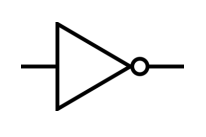
\includegraphics[height=2.5cm]{images/not.png}
        \caption{Representación gráfica de la compuerta NOT.}
    \end{figure}
    \begin{table}[H]
        \centering
        \begin{tabular}{cc} \hline
            A & NOT(A)\\ \hline
            0 & 1 \\
            1 & 0 \\ \hline
        \end{tabular}
        \caption{Compuerta clásica NOT.}
    \end{table}
\end{minipage}
\begin{minipage}{0.5\linewidth}
    \begin{figure}[H]
        \centering
        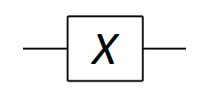
\includegraphics[height=2.1cm]{images/not_c.png}
        \caption{Representación gráfica de la compuerta cuántica NOT.}
    \end{figure}
    \begin{table}[H]
        \centering
        \begin{tabular}{cc} \hline
            A & NOT(A) \\ \hline
            $\left| 0 \right\rangle$ & $\left| 1 \right\rangle$ \\
            $\left| 1\right\rangle$ & $\left| 0 \right\rangle$ \\
            $\left| \psi \right\rangle$ & $\hat{X}\left| \psi \right\rangle$ \\ \hline
        \end{tabular}
        \caption{Compuerta cuántica NOT.}
    \end{table}
\end{minipage}
\subsubsection{Compuerta de Hadamard}
La compuerta de Hadamard opera únicamente sobre un qubit, y realiza la operación de un cambio de base, de pasar de la base $\lbrace\left| 0 \right\rangle ,\left| 1 \right\rangle\rbrace$ a la base $\lbrace\left| + \right\rangle ,\left| - \right\rangle\rbrace$
\begin{align*}
    \left| 0 \right\rangle &\underset{\hat{H}}{\rightarrow} \frac{\left| 0 \right\rangle+\left| 1\right\rangle }{\sqrt{2}} \equiv \left| + \right\rangle\\
    \left| 1 \right\rangle &\underset{\hat{H}}{\rightarrow} \frac{\left| 0 \right\rangle-\left| 1\right\rangle }{\sqrt{2}} \equiv \left| - \right\rangle\\
\end{align*}
    donde:
    \begin{equation*}
        \hat{H} = \frac{1}{\sqrt{2}} \left(\begin{matrix}
            1 & 1 \\
            1 & -1
        \end{matrix} \right)
    \end{equation*}
    Esta compuerta es usada comunmente para generar superposiciones a partir de los estados base computacional, esta se puede observar que crea una rotación de $\pi$ alrededor del eje XZ.
    \begin{figure}[H]
        \centering
        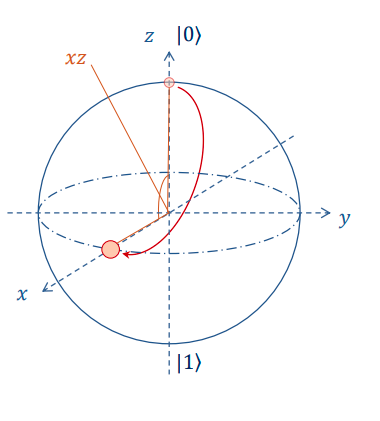
\includegraphics[scale=0.3]{images/hadamard.png}
        \caption{Representación gráfica del efecto de la transformación de Hadamard aplicada a un qubit.} 
    \end{figure}
\subsubsection{Compuerta de desplazamiento de fase}
La compuerta de desplazamiento de fase aplica unicamente a un qubit de tal forma que al estado $\left|0 \right\rangle$ lo deja intacto, pero al estado $\left|1 \right\rangle$ , lo lleva a $e^{i\theta}\left|0 \right\rangle$. Por lo que la probabilidad de medir 
cualquier estado no cambia al aplicar esta compuerta, sin embargo, sí modifican la fase del estado cuántico.
\begin{align*}
    \left| 0 \right\rangle &\underset{\hat{R}(\phi)}{\rightarrow} \left| 0 \right\rangle\\
    \left| 1\right\rangle &\underset{\hat{R}(\phi)}{\rightarrow} e^{i\phi}\left| 1\right\rangle\\
\end{align*}
    donde:
    \begin{equation*}
        \hat{R}(\phi) = \left[\begin{matrix}
            1 & 0 \\
            0 & e^{i\phi}
        \end{matrix} \right]
    \end{equation*}
    por lo que $\phi$ es el desplazamiento. Algunos casos comunes de estas puertas son la puerta $\frac{\pi}{8}$ donde $\phi=\frac{\pi}{4}$, la puerta de fase donde
    $\phi=\frac{\pi}{2}$ y la puerta de Pauli-Z donde $\phi=\pi$.
\subsubsection{Compuerta SWAP}
La compuerta SWAP es una operación de dos qubit. Expresado en estados base $|00\rangle, |01\rangle, |10\rangle, |11\rangle$. La compuerta SWAP intercambia el estado de los dos qubits involucrados en la operación. Esta representada por la matriz:\\
\begin{minipage}{0.5\linewidth}
\begin{equation*}
    U_{SWAP}=\left[\begin{matrix}
    1 & 0 & 0 & 0\\
    0 & 0 & 1 & 0\\
    0 & 1 & 0 & 0\\
    0 & 0 & 0 & 1\\
    \end{matrix}\right]
\end{equation*}
\end{minipage}
\begin{minipage}{0.5\linewidth}
\begin{figure}[H]
        \centering
        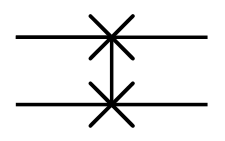
\includegraphics[scale=0.7]{images/swap_gate.png}
        \caption{Representación gráfica de la compuerta SWAP.}
    \end{figure}
\end{minipage}
\subsubsection{Compuertas Controladas}
Las puertas controladas operan sobre 2 qubits o más, de los cuales uno o más controlan la operación. Por ejemplo, la puerta NOT controlada (o CNOT) opera sobre 2 qubits, y realiza la operación NOT en el segundo qubit solo cuando el primer qubit es  $|1\rangle$ , y en otro caso lo deja intacto. Se representa por la matriz
\begin{minipage}{0.5\linewidth}
\begin{equation*}
    U_{CNOT}=\left[\begin{matrix}
    1 & 0 & 0 & 0\\
    0 & 1 & 0 & 0\\
    0 & 0 & 0 & 1\\
    0 & 0 & 1 & 0\\
    \end{matrix}\right]
\end{equation*}
\end{minipage}
\begin{minipage}{0.5\linewidth}
\begin{figure}[H]
        \centering
        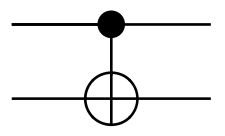
\includegraphics[scale=0.7]{images/not_gate.png}
        \caption{Representación gráfica de la compuerta NOT controlada.}
    \end{figure}
\end{minipage}